% BP-Evolve: Auditing the CBP-NG Score inside an Agentic Design Loop
% Build:  tectonic vfs_report_4p.tex   (or pdflatex twice)
% Needs:  IEEEtran.cls, amsmath, booktabs, pgfplots (all standard, all on
%         Overleaf).  No external figure files.
% Target: A^3 workshop / CHIA hackathon, 4 pages excluding references.
%         Body is exactly 4 pages; the bibliography starts on page 5.
% Cut from vfs_report.tex to meet the 4-page limit: the bounds-arm section
% ("An LLM on the Search Space" + its table) and the loop diagram (Fig. 1,
% loop.pdf) were dropped; sections III-V were compressed by roughly 20%.
% The gem5 tier (Tier 2) was then removed entirely, along with the
% "each tier must separate its population" contribution it supported; the
% loop is now two-tier (CBP-NG + ChampSim port check).
% The 6-page version is vfs_report.tex; the 9-page one is in git (59fd1b5).
%
% 2026-09-24 review pass (three independent reviews, all findings re-verified
% against the lineage DBs and the agent transcripts before being applied):
%  * The design prompt DID describe ahead-pipelining from generation 11 (971-line
%    prompt, "What the CBP-NG 2025 winners did", gshareN_ahead source inlined;
%    out_design_llm sweeps.note records it).  The "discovery" framing has been
%    removed from the abstract, the intro and Sec. V-C; the operator-reach claim
%    (which is what the loop actually tests) stands.
%  * "Widest empty band" was false: three evaluated designs lie inside
%    T in (6.87, 7.72).  Replaced with the P2 separation over all 191 evaluated
%    designs (P2>=2 max 6.870, P2<=1 min 6.955, zero overlap), which is stronger.
%  * The 126-run-to-end vs 168@4e7 offset is -0.72 +- 0.16%, not -0.92 +- 0.13%
%    (the latter is the trace-count leg alone, dropping the +0.20% window leg).
%  * Tier 1 runs on 8 traces at a 2e6-instruction window, not on 126; the
%    "MPKI 1.5-8.8% lower" range is not reproducible from the DBs and is gone.
%  * Table II's design column was computed from pre-rescore depth_scores;
%    recomputed from the rescored counters (reproduces stored VFS to 3e-16).
%  * Disclosed: held-out fraction is 0 from generation 15, so 0.9895 is
%    in-sample while gen014_0's 0.9817 is not; CPI_REF is frozen at D=9.
%
% Third pass (B1, full-population Kendall tau).  Table II ranks ELITES only --
% 21, 21 and 153 pairs -- so it measures the archive, not the operator.  Re-
% ranking every evaluation instead (122 param, 69 design; mpi=mpki/1000,
% cpi(D)=mpi*(D+p2-max(1,min(p1,p2))), vfs.vfs(ipc,cpi,epi)) gives
%    param  n=122 frozen  D=3..30: +.921 +.978 +.980 +.934 +.776 +.734
%    design n=69  frozen  D=3..30: -.371 +.452 +.839 +.782 +.754 +.742
%    design n=69  scaled  D=3..30: +.290 +.813 +.891 +.822 +.769 +.750
% so the parameter arm is NOT depth-invariant off the elite set, and the design
% population inverts at D=3.  The inversion is present in both the 126-trace
% (n=12, -0.212) and 168-trace (n=57, -0.406) subsets, so it is not a
% measurement-condition artefact; about half of it is the frozen-reference
% convention.  Section III-C now says this and the elite claim is qualified.
% Space for it came from prose compression in III-C, IV, V-B/C and VI, and from
% running the Acknowledgment in rather than giving it a heading.
%
% Third pass also carries B2 (offline selection replay).  Holding the proposal
% sequence fixed and re-running the archive's "keep the best in each cell" rule
% at other depths -- cells are (EPI band, P1, P2) and so depth-independent --
% gives, against the D=9 archive:
%    design (69 evals, 11 own cells): D=3 6 elites change, best gen018_0
%      (1.0211) not gen029_1; D=6 4 change, best gen033_1; D>=12 none change.
%    param  (90 evals,  7 cells):     D=3 4 change, best gen035_1; D=6 3 change,
%      best gen039_0; D=12 1; D=16/25/30 3 each, best stays gen037_2.
% Reported in III-C as "selection moves designs and not only ranks".  Note the
% design arm's 11 cells here are its own evaluations only; the 18-cell archive
% includes the 7 trunk designs, which live in a different database.
%  * Second pass: 71 built / 69 ran (not "69 built and ran"); gen037_2 moves
%    four of eight parameters, not one; Fig. 2 gained the two parameter-arm
%    elites it had been missing (gen014_1, gen032_1); the fork is announced in
%    Sec. II instead of first appearing in Sec. IV; ELM and FunSearch cited;
%    "116 TAGE configurations" scoped to the parameter arm (116 distinct ids,
%    122 evaluations -- ids repeat across resumed sweeps); and crossing the P2
%    separation is now distinguished from leaving the score's rising side
%    (gen018_0 is above the separation at T=7.72 with elasticity +0.244).
%    NOT applied: a reviewer claim that Dang's C is back-solved -- Dang reports
%    CPI 0.052 (prompts/cbpng_winners/3_dang.md), so the dagger stays on MORSL
%    alone, which reports no CPI.
%
% Numbers for other work (Table I, Fig. 2) are the authors' own reported
% IPC/CPI/EPI, pushed through the official vfs.py formula: Fan and Dang reproduce
% their reported VFS to 4 decimals; MORSL reports no CPI, so its CPI (0.04324) is
% back-solved from its VFS; Pallan's Table I reproduces 0.9346 (reported 0.9345).
%
% B6 (sensitivity band for the daggered row).  MORSL DOES report EPI (524
% fJ/inst, 1_morsl.md:4), so back-solving C from its VFS is identified, not a
% free parameter.  Sweeping that EPI +/-20% (419/524/629) gives
% C = 0.04456/0.04324/0.04188 and dT = +0.0010/-0.0071/-0.0159, so the row's
% sign claim ("near zero or reversed at the winning entries") survives the whole
% band.  The earlier caption said "+0.03 to -0.03 across a plausible EPI range",
% which treated EPI as unknown; it is not, and the caption now says so.  Every
% Table I row was re-derived this pass and matches to the printed digits:
% MORSL (8.647, 0.04324, 524) -> 0.9935, dT -0.007, dC -0.048, dEPI -0.007;
% Fan (8.893, 0.04705, 312.6) -> 0.9921, -0.015, -0.051, -0.005;
% Dang (8.62, 0.052, 1068) -> 0.9738 vs reported 0.9742 (CPI has 2 s.f.),
% dT +0.057, dC -0.083, dEPI -0.016.
%
% B5 (can the parameter box reach P2<=1 at all?).  Latency is structural: it is
% max over predictions of (p2_time - time) in cbp.hpp:220, independent of trace
% and of run length (verified: 200k vs 2M instructions, and two traces, give the
% same 1.36 cycles).  So each config needs one 10-second build
%   g++ -std=c++20 cbp.cpp -lz -O3 -DPREDICTOR='tage<LOGLB,NUMG,...>'
% and one 0.7-second run.  All 256 corners of the eight-parameter box (bounds
% from agents.py _TAGE_PARAMS) plus 512 random interior points (seed 20260924)
% were built and timed: P2 ranges 1.32-2.81 cycles, none at or below 1.00, so
% every one rounds up to 2.  Fastest is tage<5,4,9,10,8,40,16,10> at 1.32
% cycles = 396 ps against the 300 ps clock (cbp.hpp:12).  Raw output is in the
% job scratch dir (corners_out.txt, interior_out.txt).  Section IV now says
% "and cannot" rather than only "never reached".  The organisers'-references
% sentence (gshareN/bimodalN above the band, tage/gshare below) was cut to pay
% for this; it is weaker evidence for the same point.
%
% Section IV reweighting (2026-09-25).  The section's claim is operator reach --
% an operator that writes source can reach a design an operator that resizes
% eight integers cannot represent -- but the limitations ran to five paragraphs,
% longer than the result, and a reader met "we told the agent the answer" before
% meeting the answer.  IV-A now leads with the claim and carries the B5 probe as
% its evidence (the box is enumerable precisely because latency is structural),
% and the limitations are two paragraphs: the knowledge asymmetry first, on its
% own, then everything else as bookkeeping.  Nothing was dropped -- the five
% paragraphs' content is all still there -- and IV is 1041 words against 1054.
% Trimmed to hold four body pages: "a property of the compiled predictor rather
% than of a trace" -> "structural, invariant to the trace"; the gen022_2
% displacement compressed to a parenthesis; "and resumed sweeps"; "with that
% offset stated".
%
% Section IV removed entirely (2026-09-25, at the author's instruction).  The
% section claimed operator reach: the parameter operator rewrites eight integers
% and provably cannot reach P2<=1 (the B5 probe above), while the design agent
% crossed in one generation.  That claim, the P2-crossing narrative, the
% "what the agent did not do" plateau analysis and the five-then-two-paragraph
% limitations are all gone.  The paper is now purely an audit of the score.
% What had to move rather than die, because the rest of the paper uses it:
%   * the fork and the two arms are defined in Sec. II, with tab:stages moved
%     there; its footnote absorbs the 126-vs-168 offset and the in-sample
%     disclosure that were in Sec. IV's limitations.
%   * the P2 separation (124 designs <=6.870, 67 >=6.955, no overlap) survives
%     as one descriptive sentence in Sec. II, because Fig. 2's shaded strip is
%     otherwise unexplained.  No claim is drawn from it.
%   * the single-seed / shared-trunk / Tier-1-parameter-arm-only caveats moved
%     to the Discussion's last paragraph.
% Dropped with the section and NOT relocated: the 71-proposal build/run tally,
% gen011_0 and gen016_2, the archive plateau, the gen014_0 -> gen029_1
% accuracy-not-bandwidth analysis, the prompt digest disclosure, the /tmp
% contamination and the 68-vs-71 count.  The third contribution in the abstract
% and intro is now B2 (selection replay) instead of the crossing.
% Body is 566 lines against the 665-line four-page baseline: the bibliography
% now fits on page 4 and about one page of body space is free.
%
% Four-arm comparison added as the new Sec. IV, "What Moves the Ceiling"
% (2026-09-25), filling the page that deleting the old Sec. IV freed.  This is
% the comparison the old section was missing: it has the ablations.  Five
% operators, all scored on the 126 search traces run to completion, from the
% lineage DBs in ~/bp_evolve_data:
%   trunk    out_gcp+out_resume   rule, 2 of 8 params, gens 0-10, n=33,
%                                 best gen007_2 0.92564 T 6.84, P2<=1: 0
%   offline  out_gen50 sw 1/3/4   rule, gens 11-39, n=90,
%                                 best gen037_2 0.92884 T 6.87, P2<=1: 0
%   params   out_params           LLM picks all 8, fixed box, gens 0-14, n=43,
%                                 best gen004_2 0.92270 T 6.67, P2<=1: 0
%   bounds   out_bounds_rule      --bounds-rule 0.25, gens 11-20, n=30,
%                                 best gen014_2 0.92878 T 6.87, P2<=1: 0
%   bounds   out_bounds_llm       --tune-bounds,  gens 11-20, n=30,
%                                 best gen014_2 0.92878 T 6.87, P2<=1: 0
%   design   out_design_llm       LLM writes source, gens 11-14, n=12 (the
%                                 126-trace subset), best gen014_0 0.98384
%                                 T 8.97, P2<=1: 11 (gen011_0 is the degenerate)
% The two bounds arms reach the SAME vector 7,8,11,14,11,102,14,8 at gen 14;
% the fixed-box control reaches 7,8,11,14,12,100,14,7 (+5.8e-5) at gen 16.  The
% arms are RNG-paired and still diverge in 10 of 30 proposals, so the identical
% best is not an artefact of sharing a stream.  bound_changes: rule 2, llm 12;
% 11 of the llm's 12 NARROW the box, and its one expansion (LOGLB 7->8) is
% unused -- LOGLB histograms are {6:17,7:73}, {5:3,6:5,7:34}, {6:8,7:22},
% {6:8,7:22}, so no design in any arm ever used LOGLB=8.
% 226 = 33+90+43+30+30 parameter-space evaluations, zero with P2<=1.  Some
% vectors repeat between arms; the table reports per-arm counts, and the text
% says "not one of the 226", which holds either way.
% The B5 box enumeration returns here as the reason "none could have".
% Sec. II's arm paragraph and tab:stages were replaced by a two-sentence
% forward reference, since tab:arms supersedes them; the abstract and intro now
% claim four contributions.
% Three-reviewer pass (2026-09-25).  Corrections applied, each re-verified
% against the lineage DBs before editing:
%  * bounds/control: gen016_2 in out_gen50 sw4 is the SAME vector 7,8,11,14,
%    11,102,14,8 at the SAME score 0.92878203970762674 as both bounds arms'
%    gen014_2.  The +5.8e-5 design (7,8,11,14,12,100,14,7) is gen037_2, at
%    generation 37, not 16.  Also: launch_bounds_local.sh records an RNG
%    relaunch that offsets arm vs control by one generation from gen 12 on,
%    so the "two generations" claim was not like-for-like; both facts now
%    stated.
%  * bound_changes in out_bounds_llm: 12 accepted, of which 3 WIDEN (LOGLB
%    5-7 -> 5-8 gen 11; GHIST1 4-10 -> 2-10 gen 11; LOGB 10-14 -> 10-15 gen
%    15) and 9 narrow.  Was "eleven of twelve narrowed".  out_bounds_rule's
%    two changes are BOTH widenings and one of them is the identical LOGLB
%    5-7 -> 5-8, so the LOGLB=8 ceiling was not the agent's alone.
%  * bounds arms ran generations 11-20 = ten generations, not five.
%  * five parameter-space arms (33+90+43+30+30 = 226), not four.
%  * Sec. III-C uses three archives built by two operators, not two archives.
%  * Tier 1: the 10% gate is port_selfcheck_mpki over Tier 0's own 126 traces
%    and window with no simulator on either side (constants.py:164,178,
%    evaluator.check_port_fidelity).  The 8-trace/2e6 ChampSim run is the
%    simulation, not the gate, and disagrees with Tier 0 by >100%.  Sentence
%    rewritten.  tier=1 rows are 41 for the trunk+offline loop (gcp 2 +
%    resume 9 + gen50 30), not 42.
%  * Dang: vfs(8.62,0.052,1068) = 0.97385, dT +0.0569, dC -0.0831.  Table now
%    prints 0.9738/+0.057/-0.083 with the reported 0.9742 in the caption.
%  * Fig. 2's shaded strip was the retracted "widest empty band" (6.87,7.72);
%    three evaluated designs lie inside it.  Redrawn at the true P2 separation
%    (6.870, 6.955), and the explanatory sentence -- 192 evaluations, 125 with
%    P2>=2 at most T=6.870, 67 with P2<=1 from T=6.955 -- restored in Sec. IV,
%    which is what the caption forward-references.
%  * Sec. III-C full-population tau: the DBs hold 123 ran Tier-0 evaluations
%    in trunk+offline, not 122, and give +0.976 at D=6 and +0.723 at D=30
%    (was +0.978/+0.734).
%  * Sec. III-B "at least 9.00" -> 8.99 (gen001_2 is 8.9963).
%  * Abstract's elasticity range was scoped to the 116; over all 226 it is
%    0.278-0.747 with T down to 3.083, so the abstract now says +0.28..+0.75.
%  * Abstract's "enumerating the box" was false: 768 of 5.97e7 integer points.
%    Reworded to "probing ... all 256 corners and 512 interior points", and
%    Sec. IV now says the bounds arms' moved boxes went unprobed.
% Disclosures restored or added:
%  * 0.9895 is in sample (BPE_HELD_OUT_FRACTION=0 from gen 15); lost when
%    tab:stages was deleted.  Now in tab:arms' caption and the Discussion.
%  * out_heldout_design_design/heldout.log: the design arm's 3-elite held-out
%    test returned tau=+0.333, below the 0.6 declared in Sec. II.  Now in the
%    Discussion.
%  * the design agent alone had the winners' digest, a CBP-NG checkout and a
%    compiler (transcripts in out_design_llm/designs/*/transcript.md show it
%    reading /tmp/work/cbp and gshareN_ahead.hpp and invoking g++), so
%    representation and knowledge changed together -- Sec. IV says the
%    experiment cannot separate them, and concedes that the arm's first
%    post-fork proposal is the one exception to P2<=1.
% A hermetic replay of generations 11-14 with the winners' material deleted
%    (prompts/design_noref.md, launch_design_noref.sh, out_design_noref/) was
%    run on 2026-09-25 and is NOT reported: its control is confounded three
%    ways and cannot support a causal claim.  (a) It was built from the
%    301-line working-tree design.md, not the 170-line prompt the treatment
%    used at gens 11-14 (commit 2bb9128); the extra section 'Where the
%    remaining score is: accuracy' told the agent latency had nothing left to
%    give, which is false of the archive it was handed (best gen007_2 has
%    P2=2), and the control obeyed it -- MPKI 5.00-5.38 against the
%    treatment's 5.80-9.50, EPI 1386-2027 against 84-1111, every variant at
%    P2>=2.  (b) The control prompt dropped the 'one RAM read or write per
%    cycle' warning, the exact rule its three run failures died on.  (c) The
%    control was told no CBP-NG checkout exists and not to read /tmp, while
%    the treatment compiled against one.  Redoing it means the 170-line
%    prompt minus only its two winner sections, same rule text, same tools.
%  * llm-params moves as many parameters as it likes where the rule moves two
%    (launch_params_local.sh), so it differs in step size as well.
% Coherence: "parameter arms"/"design arm" are now defined in Sec. II (they
% were defined only in the deleted Sec. IV); tab:arms' rows renamed to match
% Tables I-II (offline -> param., params -> llm-par.); the Gens column moved
% into the caption to clear a 25pt overfull hbox; "ceiling" given a value.
% Body is 4 pages excluding references (bibliography runs onto page 5).
\documentclass[conference]{IEEEtran}
\usepackage[T1]{fontenc}
\usepackage{amsmath,amssymb}
\usepackage{booktabs}
\usepackage{balance}
\usepackage{pgfplots}
\pgfplotsset{compat=1.16}
\usepackage[hidelinks]{hyperref}

\setlength{\textfloatsep}{8pt plus 2pt minus 2pt}
\setlength{\floatsep}{8pt plus 2pt minus 2pt}
\setlength{\intextsep}{8pt plus 2pt minus 2pt}
\setlength{\abovecaptionskip}{4pt}
\setlength{\belowcaptionskip}{0pt}


\newcommand{\vfs}{\text{VFS}}
\newcommand{\mpki}{\text{MPKI}}
\newcommand{\epi}{\text{EPI}}

\begin{document}

\title{BP-Evolve: Auditing the CBP-NG Score\\inside an Agentic Design Loop}

\author{\IEEEauthorblockN{JianYu Shen}
\IEEEauthorblockA{\textit{SiFive}\\
jian-yu.shen@sifive.com}
\and
\IEEEauthorblockN{WeiCheng Lin}
\IEEEauthorblockA{\textit{National Yang Ming Chiao Tung University}\\
410011max@gmail.com}}

\maketitle

\begin{abstract}
A recent autonomous campaign tuned the CBP-NG reference TAGE predictor to a
\vfs{} of 0.9345 and concluded that, under this metric, throughput matters more
than accuracy; the winning entries reached 0.974--0.994 by a different route.
We ask what such a search is actually optimizing, using a two-tier loop on
CHIA (CBP-NG and a ChampSim port check) to run six MAP-Elites searches over the
reference TAGE that differ only in what each proposer may change. Throughput
dominance turns out to be a property of the operating region rather than of the
metric: the throughput elasticity of \vfs{} lies between $+0.28$ and $+0.75$ for
every design our parameter searches reached, yet falls to between $-0.02$ and $+0.06$ at the
winning entries, where accuracy matters $1.5$--$7\times$ more. We then ask what
that costs a search whose score is read at one pipeline depth. Re-scoring the
same counters at other depths is free, and whether a ranking survives the change
is governed by how widely a population spreads in accuracy --- the very term the
rising side of the score teaches a search to discount.
The effect is not confined to ranks: replaying the archive's own selection rule
at other depths, with the proposal sequence held fixed, changes which designs
are kept and which design is best. Finally, we run five operators on the same
problem, differing only in what each may change. Widening the search box, by
threshold or by an agent, and replacing the proposer with an agent both leave
the ceiling exactly where it was; across $226$ evaluations no operator confined
to parameters reaches the second-level latency the winning entries rely on, and
probing the template's box directly --- all $256$ corners and $512$ interior
points, compiled and timed --- leaves the fastest of them $32\%$ short. Only
writing the source does.
\end{abstract}

\section{Introduction}

Agentic and evolutionary design loops~\cite{alphaevolve,funsearch,elm,archgym}
can only be as good as the objective they optimize. Search is notoriously
literal: it finds what a score rewards, not always what the score's designers
intended~\cite{lehman2020surprising,amodei2016concrete}. Branch prediction is an
unusually clean setting in which to study this gap. The Next-Generation
Championship in Branch Prediction (CBP-NG)~\cite{cbpng} provides a simulator,
168 traces, and a reference TAGE predictor~\cite{seznec2006tage,seznec2011tage}
written in HARCOM~\cite{harcom}, a restricted dialect of C++ from which each
predictor's latency and energy are derived. Entries are ranked by
\vfs{}~\cite{vfsmetric}, which corrects a long-standing weakness of misprediction
rate: it favors predictors too slow or too power-hungry to
build~\cite{jimenez2000delay,jimenez2003reconsidering}.

Coding agents have already been turned loose on this objective.
Pallan~\cite{pallan} directed two agents through more than 2,300 configurations
of the reference TAGE. The campaign reached 0.9345, attributed most of its gain
to a single change in block length, concluded that throughput dominates accuracy
under \vfs{}, and plateaued without discovering a new architecture. The three
winning entries~\cite{koizumi,fan,dang} reached 0.974--0.994 with
ahead-pipelined designs. The lesson the agents learned may be a property of
\vfs{} itself, or only of the region in which they searched.

We audit both the score and the loop that optimizes it, and make four
contributions. First, we derive the elasticities of \vfs{} in closed form and
show that throughput dominance holds only on the rising side of the score ---
the low-throughput region in which every parameter-search design lies --- and
falls to near zero or reverses at the winning entries. Second, we show that whether that ranking
survives a change in pipeline depth is governed by how widely the archive
spreads in accuracy, and that Eq.~\eqref{eq:cpi} makes the test free.
Third, we show that the instability is not confined to how designs are ranked:
replaying the archive's selection rule at other depths, with the proposal
sequence held fixed, changes which designs it keeps and which one it calls
best. Fourth, we compare five operators that differ only in what the proposer
may change --- a rule-based proposer, an agent that chooses all eight
parameters, two that may widen the search box (one by threshold, one by an
agent), and one that lets an agent write the predictor's source --- and find
that neither a wider box nor a cleverer proposer moves the ceiling, while the
representation does. Because two of the three archives the depth audit compares
were built by a non-LLM operator, what it measures is the objective rather than
a model's priors. The loop, which connects two
toolchains through a shared lineage database on CHIA~\cite{chia}, is open source.

\section{The Design Loop}
\label{sec:loop}

The loop is a graph of CHIA nodes, each bound to its own container image and
machine pool, through which candidates pass two evaluation tiers of increasing
cost. A proposer draws a parent uniformly from the archive's occupied cells and
emits a variant; the variant is linted, built for both toolchains, run through
the tiers, and folded into a behavior descriptor. The lineage database is the
only state the toolchains share.

Tier~0 scores every variant in the CBP-NG simulator. The harness invokes the
predictor once per instruction, but a design may declare that consecutive
instructions share one lookup, a \emph{block}. Because one block retires per
cycle, prediction throughput $T$ measures front-end bandwidth, and the most
direct way to raise it is to cover more instructions per lookup. HARCOM charges
every operation the delay and energy of its circuit (ASAP5, 300\,ps clock),
yielding the latencies $p_1,p_2$ of the two prediction levels and the energy per
instruction \epi{}. Since CBP-NG imposes no storage budget, $(\epi{},p_1,p_2)$
is the entire cost model and serves as the archive's behavior grid.

Tier~1 checks that a design survives translation. A single template renders the
algorithm as a ChampSim~\cite{champsim} module, and a design is promoted only if
the rendered port, replayed over Tier~0's own traces and window with no
simulator on either side, reproduces its conditional \mpki{} to within 10\%; the
port then runs under ChampSim on eight traces at a $2\times10^6$-instruction
window. All 41 designs submitted passed, although the port departs structurally
from Tier~0 --- the first level is not ported, and ChampSim advances history per
branch rather than per block --- so the check is a portability gate, not a
second opinion on the score.

The search uses MAP-Elites~\cite{mouret2015illuminating}, which preserves
behaviorally distinct designs rather than a single incumbent. Each proposal
perturbs two of eight TAGE template parameters within declared ranges, so the
operator can resize the predictor but never change its algorithm. We ran 40
generations of three variants each, splitting the 168 traces into 126 for search
and 42 held out and simulating each to completion after $10^6$ warm-up
instructions; the best of the 116 designs improved by only 0.35\% over the last
26 generations. The held-out traces were used once, after search, in a rank
test declared in advance to signal overfitting at $\tau<0.6$.

Generations 0--10 are a shared trunk. From generation~11 the run forks into
arms that differ only in what the proposer may change: the \emph{parameter
arms}, whose proposer resizes the template within a box, and the \emph{design
arm}, whose agent writes the predictor's source outright.

\section{The Score's Two Regimes}

\vfs{} depends on only three quantities: throughput $T$,
misprediction cost $C$ (cycles lost per instruction), and \epi{}, each measured
against a hypothetical reference core with $T_\text{ref}=8$,
$C_\text{ref}=0.0315$, and $\epi{}_\text{ref}=1000$. The misprediction cost is
\begin{equation}
C = \text{mpi}\,\bigl(D + p_2 - \max(1,\min(p_1,p_2))\bigr),
\label{eq:cpi}
\end{equation}
where $D=9$ is the pipeline depth. Letting $w=TC$ denote the wrong-path
instructions fetched per retired instruction, the speedup term can be rewritten
as a ratio of \emph{useful} fetch bandwidth,
\begin{equation}
S = \frac{T/(1+w)}{T_\text{ref}/(1+w_\text{ref})},
\label{eq:speedup}
\end{equation}
and the score becomes
\begin{equation}
\vfs{} = S\cdot F(SE),\quad
F(P)=\alpha\Bigl(1-\frac{2}{1+\sqrt{1+\beta/P}}\Bigr),
\label{eq:vfs}
\end{equation}
where $E=(\rho\,\epi{}/\epi{}_\text{ref}+\lambda S^{\gamma})(1+w/2)$ and
$\rho=0.05$ is the predictor's share of core energy~\cite{vfsmetric}.

The constants follow from the delay model $f/f_0=\alpha-(\alpha-1)V_0/V$ under a
fixed power envelope $PV^2f=1$: $\alpha=1.625$ is a frequency ceiling, $\beta$
gives $F(1)=1$, and $\gamma=2/(\alpha-1)=3.2$ makes $S^\gamma$ the DVFS energy of
running $S$ times faster. \vfs{} is thus the speedup at fixed frequency times
the clock rate its power budget permits. Our reimplementation reproduces the
reference score, every stored score, and other entries' reported scores
(Table~\ref{tab:elast}).

\begin{table}[tb]
\caption{Elasticity $\partial\ln\vfs{}/\partial\ln x$ at reported operating
points. Published entries use the points given in their papers; our design-arm
rows are measured on 168 traces at $4\times10^7$ instructions, our parameter-arm
rows on the 126 search traces. $^\dagger$\,$C$ is back-solved from the reported
\vfs{} at MORSL's reported \epi{} of $524$; a $\pm20\%$ error there would move
$\partial T$ only to $+0.001$/$-0.016$. Fan and Dang report $C$; Fan's row
reproduces his published \vfs{} exactly and Dang's to three decimals ($0.9738$
against $0.9742$, his $C$ being given to two significant figures).}
\label{tab:elast}
\centering\scriptsize
\begin{tabular}{@{}lrrrrr@{}}
\toprule
Design & \vfs{} & $T$ & $\partial T$ & $\partial C$ & $\partial\epi{}$ \\
\midrule
reference & $1.0000$ & $8.00$ & $+0.008$ & $-0.035$ & $-0.013$ \\
\midrule
MORSL$^\dagger$~\cite{koizumi} (1st) & $0.9935$ & $8.65$ & $-0.007$ & $-0.048$ & $-0.007$ \\
Fan~\cite{fan} (2nd) & $0.9921$ & $8.89$ & $-0.015$ & $-0.051$ & $-0.005$ \\
Dang~\cite{dang} (3rd) & $0.9738$ & $8.62$ & $+0.057$ & $-0.083$ & $-0.016$ \\
Pallan~\cite{pallan} & $0.9345$ & $6.84$ & $+0.275$ & $-0.130$ & $-0.021$ \\
\midrule
design \texttt{gen029\_1} & $0.9895$ & $8.73$ & $+0.013$ & $-0.061$ & $-0.006$ \\
design \texttt{gen014\_0} & $0.9817$ & $8.86$ & $+0.036$ & $-0.080$ & $-0.006$ \\
design \texttt{gen018\_0} & $0.8954$ & $7.72$ & $+0.244$ & $-0.226$ & $-0.002$ \\
\midrule
param.\ \texttt{gen037\_2} & $0.9288$ & $6.87$ & $+0.278$ & $-0.135$ & $-0.024$ \\
seed TAGE & $0.8784$ & $5.80$ & $+0.410$ & $-0.149$ & $-0.024$ \\
param.\ \texttt{gen029\_2} & $0.6750$ & $3.67$ & $+0.677$ & $-0.138$ & $-0.040$ \\
\bottomrule
\end{tabular}
\end{table}

\begin{figure}[tb]
\centering
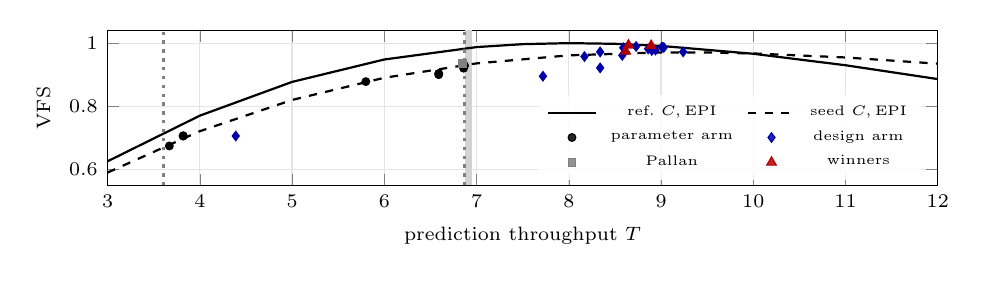
\begin{tikzpicture}
\begin{axis}[width=\columnwidth,height=3.55cm,
  xlabel={prediction throughput $T$}, ylabel={\vfs{}},
  xmin=3,xmax=12, ymin=0.55,ymax=1.04,
  legend columns=2,
  legend style={font=\tiny,at={(0.98,0.03)},anchor=south east,draw=none,
                fill=white,fill opacity=0.85,text opacity=1,column sep=3pt},
  tick label style={font=\scriptsize}, label style={font=\scriptsize},
  grid=major, grid style={gray!20}]
\fill[gray!35] (axis cs:6.87,0.55) rectangle (axis cs:6.955,1.04);
\addplot[thick] coordinates
 {(3.0,0.6264) (4.0,0.7707) (5.0,0.8774) (6.0,0.9483) (7.0,0.9875) (7.5,0.9968)
  (8.0,1.0000) (8.5,0.9979) (9.0,0.9912) (10.0,0.9664) (11.0,0.9301)
  (12.0,0.8864)};
\addlegendentry{ref.\ $C,\epi{}$}
\addplot[thick,dashed] coordinates
 {(3.0,0.5908) (4.0,0.7216) (5.0,0.8204) (6.0,0.8905) (7.0,0.9360) (8.0,0.9614)
  (9.0,0.9707) (9.5,0.9704) (10.0,0.9674) (11.0,0.9547) (12.0,0.9350)};
\addlegendentry{seed $C,\epi{}$}
\addplot[only marks,mark=*,mark size=1.4pt] coordinates
 {(3.67,0.6750) (3.82,0.7061) (3.82,0.7073) (5.80,0.8784) (6.59,0.9003)
  (6.59,0.9041) (6.86,0.9207) (6.87,0.9288)};
\addlegendentry{parameter arm}
\addplot[only marks,mark=diamond*,mark size=1.7pt,blue!65!black] coordinates
 {(4.39,0.7064) (7.72,0.8954) (8.17,0.9576) (8.34,0.9218) (8.34,0.9722)
  (8.58,0.9613) (8.59,0.9855) (8.73,0.9895) (8.86,0.9817) (8.90,0.9770)
  (8.94,0.9782) (9.01,0.9876) (9.03,0.9864) (9.24,0.9723)};
\addlegendentry{design arm}
\addplot[only marks,mark=square*,mark size=1.4pt,gray] coordinates {(6.844,0.9345)};
\addlegendentry{Pallan}
\addplot[only marks,mark=triangle*,mark size=2pt,red!70!black] coordinates
 {(8.617,0.9742) (8.647,0.9935) (8.893,0.9921)};
\addlegendentry{winners}
\addplot[gray,dotted,very thick,forget plot] coordinates {(3.61,0.55) (3.61,1.04)};
\addplot[gray,dotted,very thick,forget plot] coordinates {(6.87,0.55) (6.87,1.04)};
\end{axis}
\end{tikzpicture}
\caption{\vfs{} against $T$ with $C$ and \epi{} fixed (lines), with reported
designs (marks). Dotted lines bracket all 116 parameter-arm evaluations; its
seven elites are shown with the seed; the shaded strip is the gap between the two $P_2$
populations (Section~\ref{sec:arms}). The design arm's degenerate elite ($T=0.33$) is off
scale.}
\label{fig:tcurve}
\end{figure}

\subsection{Throughput dominance is a regime}

Table~\ref{tab:elast} shows that the score's sensitivity depends on where a
design sits. With $C$ and \epi{} at their reference values, \vfs{} peaks at
$T=8.05$, where the throughput elasticity is only $+0.008$ and accuracy
($-0.035$) is the largest term: near the reference the score is intentionally
insensitive to additional width.

The picture changes lower on the curve of Fig.~\ref{fig:tcurve}. Every design
the parameter arm produced lies in $T\in[3.61,6.87]$ with throughput
elasticities between $+0.28$ and $+0.68$, and in all 116 the throughput term
exceeds the accuracy term by $1.2$--$5.2\times$; Pallan's campaign occupied the
same region, its reported sensitivities agreeing with Eq.~\eqref{eq:vfs} to
within $0.2$ points.

The winning entries lie elsewhere: their throughput elasticities fall to between
$-0.015$ and $+0.057$ while their accuracy elasticities grow to
$-0.048$--$-0.083$, and MORSL and Fan sit almost exactly at the throughput that
maximizes \vfs{} for their own $C$ and \epi{} ($8.59$ and $8.78$), where further
width would \emph{lower} the score --- reached through
ahead-pipelining~\cite{koizumi,fan,dang}, which no resizing of the reference
TAGE can express. Throughput dominance describes the region parameter search
explores, not \vfs{} itself, and an agent that internalizes it keeps buying
width past the point at which width pays.

\subsection{Selection on the rising side}

The same effect is visible within our own population. Across the 116
configurations the rule-based arms evaluated, \vfs{} correlates with $T$ at
$r=+0.949$ but with \mpki{} at only $r=-0.113$, though \mpki{} varies from
$5.08$ to $10.08$. This arm's best design, \texttt{gen037\_2}, moves four
parameters, but the one that pays is the block length \texttt{LOGLB}, raised
from 6 to 7 --- the change Pallan's agents also found; its \mpki{} barely moves
($5.338\to5.333$) while $T$ rises from $5.80$ to $6.87$. The most accurate design here (\mpki{} $5.084$) scores only
$0.744$, and all seven final elites sit at \texttt{LOGLB}$=7$, the template's
upper bound.

Accuracy here is less a slope the search climbs than a cliff it falls from:
widening the block consumes hashed tag bits, leaving
$H=\texttt{TAGW}-(\texttt{LOGLB}-2)$, and the 100 designs with $H\ge6$ average
$5.43$ \mpki{} against $9.47$ for the 16 with $H\le5$.

\subsection{The ranking at other pipeline depths}
\label{sec:depth}

\vfs{} is read at $D=9$, but $D$ is a property of the machine and enters the
score only through Eq.~\eqref{eq:cpi}, so any depth follows in closed form from
counters measured once. We rank each archive's elites at each depth against the
ranking at $D=9$ using Kendall's $\tau$ (Table~\ref{tab:tau}): the trunk at
generation~10 and the parameter arm at generation~39, which share no designs,
and the design arm at generation~34, which contains the trunk's seven.

\begin{table}[tb]
\caption{Kendall $\tau$ of each archive's ranking at depth $D$ against its own
at $D=9$, with discordant pairs. The archives hold 7, 7 and 18 elites: 21, 21
and 153 pairs.}
\label{tab:tau}
\centering\scriptsize
\begin{tabular}{@{}rrrrrrr@{}}
\toprule
& \multicolumn{2}{c}{trunk, gen.\ 10} & \multicolumn{2}{c}{param., gen.\ 39}
& \multicolumn{2}{c}{design, gen.\ 34} \\
\cmidrule(lr){2-3}\cmidrule(lr){4-5}\cmidrule(lr){6-7}
$D$ & $\tau$ & disc. & $\tau$ & disc. & $\tau$ & disc. \\
\midrule
3  & $+1.000$ & 0 & $+0.905$ & 1 & $+0.582$ & 32 \\
6  & $+1.000$ & 0 & $+1.000$ & 0 & $+0.856$ & 11 \\
12 & $+1.000$ & 0 & $+1.000$ & 0 & $+0.935$ &  5 \\
16 & $+0.905$ & 1 & $+1.000$ & 0 & $+0.882$ &  9 \\
25 & $+0.619$ & 4 & $+1.000$ & 0 & $+0.804$ & 15 \\
30 & $+0.619$ & 4 & $+1.000$ & 0 & $+0.765$ & 18 \\
\bottomrule
\end{tabular}
\end{table}

The three archives behave very differently, and Eq.~\eqref{eq:cpi} says why:
$C\propto\text{mpi}\cdot D$, so a design with $1.7\times$ the misprediction rate
loses ground $1.7\times$ faster as $D$ grows. At generation 10 every discordant
pair involves \texttt{gen006\_2}, the only elite with high \mpki{} ($9.28$,
against $5.27$--$5.63$); removing it restores $\tau=+1$ at every depth. By
generation 39 it had been evicted, the archive's \mpki{} range had narrowed from
$1.8\times$ to $1.09\times$, and its ranking is identical from $D=6$ to $D=30$.
The design arm is the strongest case: its eighteen elites span \mpki{}
$5.26$--$11.27$ and rank least stably ($\tau=+0.58$ at $D=3$, $+0.77$ at
$D=30$). Illumination and depth robustness pull against each other, and nothing
in the depth-9 score tells the fragile archive from the robust one.

Table~\ref{tab:tau} ranks elites, so it measures the archive, not the search.
Ranking every evaluation instead --- all $123$ of the rule-based arms' and $69$
of the design arm's --- removes that selection, and the stability goes with it:
the parameter population is not depth-invariant either ($\tau=+0.976$ at $D=6$,
$+0.723$ at $D=30$), and the design population inverts outright at $D=3$
($\tau=-0.371$), in the 126- and 168-trace subsets alike. Half of the inversion
is a convention: Eq.~\eqref{eq:cpi} deepens each design's misprediction cost
with $D$ while the reference core stays at $D=9$, and scaling the reference too
gives $\tau=+0.290$ at $D=3$, leaving the archives' ordering unchanged. Replaying selection itself at other depths, with the
proposal sequence held fixed, moves designs and not only ranks: at $D=3$ four of
the parameter arm's seven cells and six of the design arm's own eleven would
hold a different elite, and the design arm's best would be \texttt{gen018\_0},
not \texttt{gen029\_1}. Depth stability is a property of the set that survived
selection, not of the operator.

Held-out traces preserve the generation-39 ranking exactly, every elite losing
a near-constant $0.0287\pm0.0019$.
% All numbers in this section are measured on 168 traces at a 4e7-instruction
% window, the condition used throughout the paper except where stated.

\section{The Ceiling and the Operator's Reach}
\label{sec:arms}

Every design in the rising region came from an operator that resizes eight
integers, so it is unclear whether that region belongs to the search space or to
the proposer. The loop ran five operators, differing in what the proposer may
change, and together they bound two explanations of why a parameter search stops
where it does --- here at \vfs{}~$0.929$, $T=6.87$: that the proposer is not
clever enough, or that its representation cannot express the next step.
Table~\ref{tab:arms} compares them.

\begin{table}[tb]
\caption{Five operators on the same problem. \emph{May
change} is the proposer's authority, $n$ its evaluations, \vfs{} and $T$ the
arm's best, and the last column counts those reaching $P_2\le1$; all rows are
scored on the 126 search traces run to completion, over generations 0--10,
11--39, 0--14, 11--20, 11--20 and 11--14, at unequal budgets. The trunk
precedes and is shared by \texttt{param.}\ and the bounds arms;
\texttt{llm-par.}\ runs from the seed. The design arm ran on to generation~34 on
all 168 traces at a $4\times10^7$-instruction window, reaching $0.9895$ in
sample; its seven trunk designs differ by $-0.72\pm0.16\%$ between the two
conditions.}
\label{tab:arms}
\centering\scriptsize
\begin{tabular}{@{}lllrrrr@{}}
\toprule
Arm & Proposer & May change & $n$ & \vfs{} & $T$ & \#$P_2\!\le\!1$ \\
\midrule
trunk    & rule  & 2 params    & 33 & $0.9256$ & $6.84$ & 0 \\
param.   & rule  & 2 params    & 90 & $0.9288$ & $6.87$ & 0 \\
llm-par. & agent & 8 params    & 43 & $0.9227$ & $6.67$ & 0 \\
bounds   & rule  & params, box & 30 & $0.9288$ & $6.87$ & 0 \\
bounds   & agent & params, box & 30 & $0.9288$ & $6.87$ & 0 \\
design   & agent & the source  & 12 & $0.9838$ & $8.97$ & 11 \\
\bottomrule
\end{tabular}
\end{table}

The first five rows end within $0.7\%$ of one another, and none reaches $T=7$.
The two bound-movers converge on the same parameter vector at generation~14, and
the fixed-box control evaluates that same vector, to the last digit of its
score, at generation~16; the only design it ever finds worth more --- by
$5.8\times10^{-5}$ --- arrives twenty-one generations later. Moving the bounds
bought no better design, and no clear time either.

Replacing the proposer with a model did not move it either. Given the same fixed
box, the agent that chooses all eight parameters at once ended at $0.9227$ after
fifteen generations and $43$ evaluations, behind the $0.9256$ the rule-based
operator had reached by generation~7, though it moves as many parameters as it
likes where the rule moves two. The bounds arms are the sharper test, being
paired: both resumed from the generation-10 archive under one random stream and
differed only in who moved the box. The
agent moved it far more actively --- twelve changes with written rationales
against the threshold's two --- and the populations did diverge, in $10$ of $30$
proposals. They arrived at the same best design anyway, and every
coordinate of it lies inside the original box --- two of them on its original
ceilings --- so no bound change was binding on it. Nine of the agent's twelve
changes \emph{narrowed} the box, pruning regions its own evaluations had shown
to be dead; of the three expansions, the one raising the \texttt{LOGLB} ceiling
from~$7$ to~$8$ was made by the threshold arm too, and no design in either arm
took any of them up.

What does move the ceiling is what the proposer may write. Across the $192$
evaluations of the two representations, throughput separates on $P_2$ without
overlap: the $125$ with $P_2\ge2$ reach at most $T=6.870$, the $67$ with
$P_2\le1$ start at $T=6.955$, and not one of the $226$ parameter-space
evaluations reached $P_2\le1$. Latency here is structural --- a property of the
compiled predictor, not of a trace --- so the box can be probed directly: its
$256$ corners and $512$ random interior points, compiled and timed, give $P_2$
from $1.32$ to $2.81$ cycles, the fastest $396$\,ps against a $300$\,ps clock
and still a third too slow. The bounds arms' raised \texttt{LOGLB} ceiling left
their boxes unprobed, but mean probed $P_2$ rises with \texttt{LOGLB}, from
$1.91$ at~$5$ to $2.00$ at~$7$. Reaching $P_2\le1$ needs the index computed a block ahead so the prediction is
latched when the cycle begins, an algorithmic change and not a resizing. Eleven
of the design arm's first twelve evaluations have it; the exception, its first
proposal after the fork, is a degenerate design holding a cell nothing else
reaches.

This is reach, not discovery. From generation~11 the design agent's prompt
carried a digest of the CBP-NG~2025 winning entries naming ahead-pipelining and
giving the index-early/select-late recipe, and the agent held a CBP-NG checkout
and a compiler; the parameter operators were given none of this because they
could have done nothing with it. Representation and knowledge therefore changed
together, and this experiment cannot separate them. What the five
parameter-space arms do bound is the other explanation: over ten generations of
bound-moving, a second proposer and $226$ evaluations, the ceiling does not move
at all.

\section{Discussion and Conclusion}

\vfs{} is a genuine improvement over ranking predictors by misprediction rate,
but what it rewards depends on where a design stands: below the reference
throughput it rewards width, near the reference accuracy, and a loop that
sees only the first regime draws the wrong lesson from its own success. The
throughput elasticity (Table~\ref{tab:elast}) says which regime a design is in,
and is the number we recommend an agentic search report, alongside rankings at
several depths, which Eq.~\eqref{eq:cpi} makes free. The same audit says where
such a loop stops: not at the limit of its proposer's cleverness but of what its
operator may write.

Our scores are not a comparison with the published entries: their values come
from a different trace sample and their operating points are self-reported
(MORSL's $C$ is inferred); this paper measures a loop, not an entry. The bounds
arms are RNG-paired and \texttt{llm-par.}\ shares the trunk's box and seed, but
the design arm is neither: it ran under a single seed, Tier~1 was run on the
parameter arms alone, and its held-out fraction was zero from generation~15, so
its $0.9895$ is in sample where \texttt{gen014\_0}'s $0.9817$ is not; an earlier
three-elite held-out test on it returned $\tau=+0.333$, below our declared
$0.6$. The loop is open source at \url{https://github.com/chia-hackathon/chia}.

% Acknowledgment required by the A^3 CFP; run in as a paragraph, no heading.
\noindent\textbf{Acknowledgment.} Drafted in part with AI assistance (Claude
Opus~5); the authors are responsible for it.

\balance
\begin{thebibliography}{99}
\bibitem{cbpng} A. Lindsay, P. Michaud, R. Sheikh, M. Madhav, and A. Alameldeen,
``The Next-Generation Championship in Branch Prediction (CBP-NG),'' held with
ISCA 2026. Simulator: \url{https://github.com/AmpereComputing/cbp-ng}.
\bibitem{harcom} P. Michaud, ``HARCOM: Hardware complexity model for
microarchitecture exploration,'' CBP-NG documentation, 2026.
\bibitem{vfsmetric} P. Michaud, ``A scoring metric for the CBP-NG
championship,'' CBP-NG documentation, 2026.
\bibitem{chia} A. Cui \emph{et al.}, ``CHIA: An open-source framework for
principled, agentic AI-driven hardware/software co-design research,''
arXiv:2606.27350, 2026.
\bibitem{pallan} M. Pallan, ``Coding agents as design searchers: An autonomous
TAGE tuning campaign for CBP-NG,'' in \emph{CBP-NG Workshop (ISCA)}, 2026.
\bibitem{koizumi} T. Koizumi \emph{et al.}, ``MORSL: Minimal-overhead
rank-based predictor with summation-free correction and lazy access,'' in
\emph{CBP-NG Workshop (ISCA)}, 2026.
\bibitem{fan} J. Fan, ``Enhance ahead-pipelined N-branch GShare with tagged
tables,'' in \emph{CBP-NG Workshop (ISCA)}, 2026.
\bibitem{dang} N. Dang and E. Rotenberg, ``An energy-efficient ahead-pipelined
TAGE branch predictor for CBP-NG,'' in \emph{CBP-NG Workshop (ISCA)}, 2026.
\bibitem{seznec2006tage} A. Seznec and P. Michaud, ``A case for (partially)
tagged geometric history length branch prediction,'' \emph{J. Instruction-Level
Parallelism}, vol. 8, 2006.
\bibitem{seznec2011tage} A. Seznec, ``A new case for the TAGE branch
predictor,'' in \emph{Proc. MICRO}, 2011.
\bibitem{jimenez2000delay} D. A. Jim\'enez, S. W. Keckler, and C. Lin, ``The
impact of delay on the design of branch predictors,'' in \emph{Proc. MICRO},
2000.
\bibitem{jimenez2003reconsidering} D. A. Jim\'enez, ``Reconsidering complex
branch predictors,'' in \emph{Proc. HPCA}, 2003.
\bibitem{champsim} N. Gober \emph{et al.}, ``The Championship Simulator:
Architectural simulation for education and competition,'' arXiv:2210.14324, 2022.
\bibitem{mouret2015illuminating} J.-B. Mouret and J. Clune, ``Illuminating
search spaces by mapping elites,'' arXiv:1504.04909, 2015.
\bibitem{alphaevolve} A. Novikov \emph{et al.}, ``AlphaEvolve: A coding agent
for scientific and algorithmic discovery,'' arXiv:2506.13131, 2025.
\bibitem{archgym} S. Krishnan \emph{et al.}, ``ArchGym: An open-source
gymnasium for machine learning assisted architecture design,'' in \emph{Proc.
ISCA}, 2023.
\bibitem{funsearch} B. Romera-Paredes \emph{et al.}, ``Mathematical discoveries
from program search with large language models,'' \emph{Nature}, vol.\ 625,
2024.
\bibitem{elm} J. Lehman \emph{et al.}, ``Evolution through large models,''
\emph{arXiv:2206.08896}, 2022.
\bibitem{lehman2020surprising} J. Lehman \emph{et al.}, ``The surprising
creativity of digital evolution,'' \emph{Artificial Life}, vol. 26, no. 2, 2020.
\bibitem{amodei2016concrete} D. Amodei \emph{et al.}, ``Concrete problems in
AI safety,'' arXiv:1606.06565, 2016.
\end{thebibliography}

\end{document}
